\documentclass[a4paper]{article}

\pdfoutput=1
\usepackage[utf8]{inputenc}
\usepackage[super,sort\&compress,comma]{natbib}
\renewcommand{\supercite}[1]{\cite{#1}}

%% Language and font encodings
\usepackage[english]{babel}
\usepackage[T1]{fontenc}
\usepackage{csquotes}

%% Sets page size and margins
\usepackage[a4paper,top=3cm,bottom=2cm,left=3cm,right=3cm,marginparwidth=1.75cm]{geometry}

% Useful packages
\usepackage{amsmath}
\usepackage{graphicx}
\usepackage{hyperref}
\hypersetup{colorlinks=true, allcolors=blue}
\usepackage{authblk}
\usepackage{multirow}
\usepackage{nomencl}
\usepackage{booktabs}
\usepackage{tabularx}
\usepackage{textcomp}
\usepackage{amsfonts}
\usepackage{outlines} %%same
\usepackage{subfig}
\usepackage[version=4]{mhchem}
\usepackage{siunitx}
\usepackage{bm}
\usepackage[normalem]{ulem} %%temporary, for organization purposes


\date{}
\newcommand{\red}[1]{\textcolor{red}{#1}}
\DeclareSIUnit\angstrom{\text {Å}}
\usepackage[final]{changes}


\interfootnotelinepenalty=10000
% Changed idea title idea from orignal title of
% "Towards a free high quality powder x-ray diffractogram database"
\title{The powder x-ray diffractogram open database}

\author[1,2]{Daniel Hollarek}
\author[1,2]{Henrik Schopmans}
\author[1,2]{Pascal Friederich}
\author[2]{Ben Breitung}
\author[2]{Simon Schweidler}
\author[3]{Andrea Hodge \AMD}
\author[3]{Adie Alwen}
\author[4,5]{Carolin Sutter-Fella}
\author[4]{Mriganka Singh}
\author[4]{Tim Kodalle}
\author[4]{Maged Abdelsamie}


% I made the affiliations smaller because there's a lot of them
\renewcommand\Affilfont{\small}


\affil[1]{Institute of Theoretical Informatics, Karlsruhe Institute of Technology,\protect \\
Engler-Bunte-Ring 8, 76131 Karlsruhe, Germany}
\affil[2]{Institute of Nanotechnology, Karlsruhe Institute of Technology,\protect \\ Hermann-von-Helmholtz-Platz 1, 76344 Eggenstein-Leopoldshafen, Germany}
\affil[3]{Department of Aerospace and Mechanical Engineering, University of Southern California, \protect \\3650 McClintock Ave, Los Angeles, CA 90089, USA}
\affil[4]{Department of Chemical Engineering and Materials Science, University of Southern California,\protect \\ 925 Bloom Walk, HED 216, Los Angeles, CA 90089, USA}
\affil[5]{Lawrence Berkeley National Laboratory, Molecular Foundry Division,\protect \\ 1 Cyclotron Rd., Berkeley, 94720 CA, USA}

\begin{document}



\maketitle
\begin{abstract}
Powder X-ray diffraction (pXRD) experiments are a cornerstone for materials structure characterization.
Despite its widespread application, the analysis of the diffractograms still presents a significant bottleneck
in high-throughput experimentation that remains to be solved in order to match the increased throughput
of the prior stages of experimentation. In the current landscape of powder X-ray diffraction analysis, machine learning has emerged as a promising research direction to resolve this bottleneck by enabling automated powder diffraction analysis.
A notable difficulty in applying machine learning to this domain is the lack of labeled datasets, i.e.\
diffraction patterns originating from experiment with accompanying structure solutions, which has relegated machine learning
researchers to train on simulated data.
Since these simulations largely fail to accurately reflect the experiment, the performance of models trained
on this simulated data by and large fails to transfer to experiment and provide value in practice.
We aim to remedy this by providing a freely available and easily accessible dataset of partially labeled
powder diffraction data, providing machine learning researchers with a large quantity of real experimental diffractograms collected from a broad range of samples.
We hope that this can guide machine learning research toward more realistic handling of experimental imperfections to enable the improvement of current automated analysis workflows.
\end{abstract}

\section{Introduction}\label{sec:introduction}
% High throughput experimentation
The advent of high-throughput experiments holds the prospect of significantly accelerating the speed of materials discovery\cite{Liu2019}. The synthesis and characterization of novel materials are becoming increasingly efficient and automated, increasing the throughput of samples in experimentation pipelines\cite{MacLeod2019, Ludwig2019, Ozaki2020}. \\

% On Rietveld refinement
After fabricating a new material, a number of analysis techniques can be used to characterize the sample. One method that can be used for phase identification, phase quantification, grain size characterization, and partially to determine the crystal structure of a new material is powder X-ray diffraction. To determine crystal structure from pXRD data, an initial guess is optimized using Rietveld refinement. In this process, an initial crystal structure including unit cell parameters is provided by the operator of the analysis software and fitted to the observed diffractogram in an iterative optimization process based on simulated forward prediction of expected pXRD diffractograms given the current crystal structure\cite{Dinnebier2019, Cano2021}. As Rietveld refinement is a local optimization method, the result of the refinement procedure is only as good as the initial guess it was provided with. \\

% Manual vs (ML) automated Refinement
Manually performing Rietveld refinement is time-consuming and often requires expert knowledge. It is not scalable to the degree required to keep up with advances in throughput and efficiency in other steps of the experimentation pipeline. In a Rietveld refinement process, the operator starts by setting parameters that characterize the background and peak shape of the powder diffraction pattern and determining a crystal structure from which the optimization process can start. The latter is usually done using search-match software, which identifies crystal structures with similar powder diffraction patterns from a database of crystal structures with accompanying powder diffraction patterns. However, attempting to refine all crystal structure parameters at once, starting from this initial structure, is known to lead to unphysical results. What makes the refinement process time-consuming and difficult is finding the correct order in which to refine the crystal structure parameters\cite{Ozaki2020}.  Additionally, if the fit develops into an unphysical set of parameters in this iterative determination of parameters, the operator must intervene to backtrack to the last step. \\

Commonly used databases for obtaining a match include the Powder Diffraction File\cite{GatesRector2019}, the Inorganic Crystal Structure Database \cite{Belsky2002}, and the Crystallography Open Database \cite{Grazulis2009}. An initial guess obtained from such a database is by no means guaranteed to lead to an accurate structure solution, even if it is iteratively revised, either manually or using blackbox optimization\cite{Ozaki2020}. Especially for novel observed structure types, simply matching to a database of known structures will not yield good results. Therefore, more complex crystal structure solution approaches need to be applied to find suitable crystal structure guesses. \\


Machine learning has the potential to speed up the manual analysis of powder diffractograms and keep pace with an automated high-throughput experimentation environment\cite{Agrawal2019, Surdu2023}.
Models can be trained to predict crystal structure information directly given a diffractogram, or models can be used to automate the conventional workflow of finding an initial guess \cite{Surdu2023} and running ML-automated Rietveld refinement \cite{Feng2019}.
So far, however, due to an absence of labeled datasets with experimental diffractograms\cite{Wang2020}, machine learning in this domain has largely relied on diffractograms simulated from known structures\cite{Park2017, Lee2023} or, most recently, from generated synthetic crystals\cite{Schopmans2023}. \\

% Predicting structure information with machine learning
Models trained on datasets with simulated diffractograms have already shown very strong performance in predicting lattice parameters\cite{Dong2021, Chitturi2021, Habershon2004, zhang2024crystallographic}, spacegroup \cite{Schopmans2023, Oviedo2018, Park2017, Vecsei2018, Zaloga2020, Suzuki2020, Chakraborty2021,zhang2024crystallographic}, and crystallite size \cite{Dong2021, Chakraborty2021} from simulated diffractograms.
However, the performance substantially drops off when these models are applied to data originating from experiments \cite{Schopmans2023,zhang2024crystallographic}[cite 2-3 papers, incl. ours].
The patterns observed in experiments exhibit imperfections that do not appear when simulating the X-ray diffraction pattern of a powder sample under ideal conditions. The physical effects underlying these imperfections need to be modeled accurately in order to be able to transfer models trained on simulated data to experimental patterns. Most approaches currently model these imperfections as a simple signal based on a heuristic functional form added to the simulated diffractograms.

At the moment, the number of openly available datasets for experimental powder data is very limited. The main sources for experimental patterns are XXX, YYY, and ZZZ. Further commercial datasets such as KKK and LLL exist, but license fees and restrictions in their use to train publishable models or even publish the training data limit their usability. Collecting a labeled dataset of raw experimental powder X-ray diffraction data of sufficient size to directly train a model that predicts crystal structure information is likely out of reach. The most advanced ML models currently are trained on approximately $10^7 - 10^8$ simulated diffractograms, which is - to the best of our knowledge - three orders of magnitude larger than the largest currently curated experimental dataset (PDF-5+ with approximately 20,000 experimental patterns) and even x orders of magnitude larger than the number of unlabeled diffractograms in the opXRD dataset we present here. \\

However, even small labeled and also unlabeled experimental diffractograms hold significant value in practice. First of all, labeled data can be used to better test and benchmark existing and new automated analysis approaches, which yields a better comparison than when using the very limited currently available datasets, such as the commonly used RRUFF mineral dataset\cite{Armbruster2015}. \\

Furthermore, even completely unlabeled data can enable machine learning researchers to evaluate how closely their simulations represent experimental data, identify what features are missing, and modify their simulation algorithms accordingly to arrive at a simulation that mirrors how data appears in reality. In this way, one can bring the simulated patterns closer to those observed in experiments by more accurately modeling the scattering process.
Improving the simulation of data involves accounting for more of the physical effects that influence the scattering process such as preferred grain orientation, variations in grain size, crystal defects, the impact of temperature on the scattering process, internal stress, and X-ray-induced fluorescence\cite{cao2024simxrd, Waseda2011, Pecharsky2023}.  Additionally, it should be considered that varying experimental setups can produce distinct powder diffraction patterns on the same sample. Features that may vary between experimental setups and influence the recorded pattern include the shape of diffraction peaks, the wavelength and polarization of the employed X-ray source, and the detector geometry
\cite{Waseda2011, Pecharsky2023}. Some experimental setups may also exhibit imperfections such as displacement of the sample from its intended position leading to the recorded scattering angles being slightly erroneous \cite{hulbert2023} or background events originating from instrument noise or X-rays scattering off equipment onto the screen.\\

Additionally, some of the observed imperfections, such as background and noise, can be accounted for using transfer learning approaches. In transfer learning the objective is to transfer the capabilities of a model learned on a source domain in which labeled data is abundant to a target domain in which labeled data is sparse\cite{Zhuang2021}. In this context, the source domain is simulated powder diffraction patterns and the target domain is experimental powder diffraction patterns. Many approaches to transfer learning have been proposed, particularly in the domain of image classification \cite{Gatys2016, Ganin2015}. These existing techniques could potentially be adapted to facilitate transfer learning in the context of pXRD patterns.

In this publication, we provide a new open powder X-ray diffraction (opXRD) dataset that collects a broad range of patterns from experiments, exceeding the currently available amount of openly accessible experimental patterns by XX.
Our opXRD dataset has been curated by collecting the accumulated powder data from multiple large research groups and institutions with high-throughput XRD facilities. It contains pXRD patterns from single and multiphase materials from a wide variety of materials classes, including XXX, YYY, and ZZZ. Details about the experiments of contributing research groups are discussed in this paper, along with a detailed description of how to contribute further data and how to use the data. \\

\begin{figure*}[!htb]
    \centering
    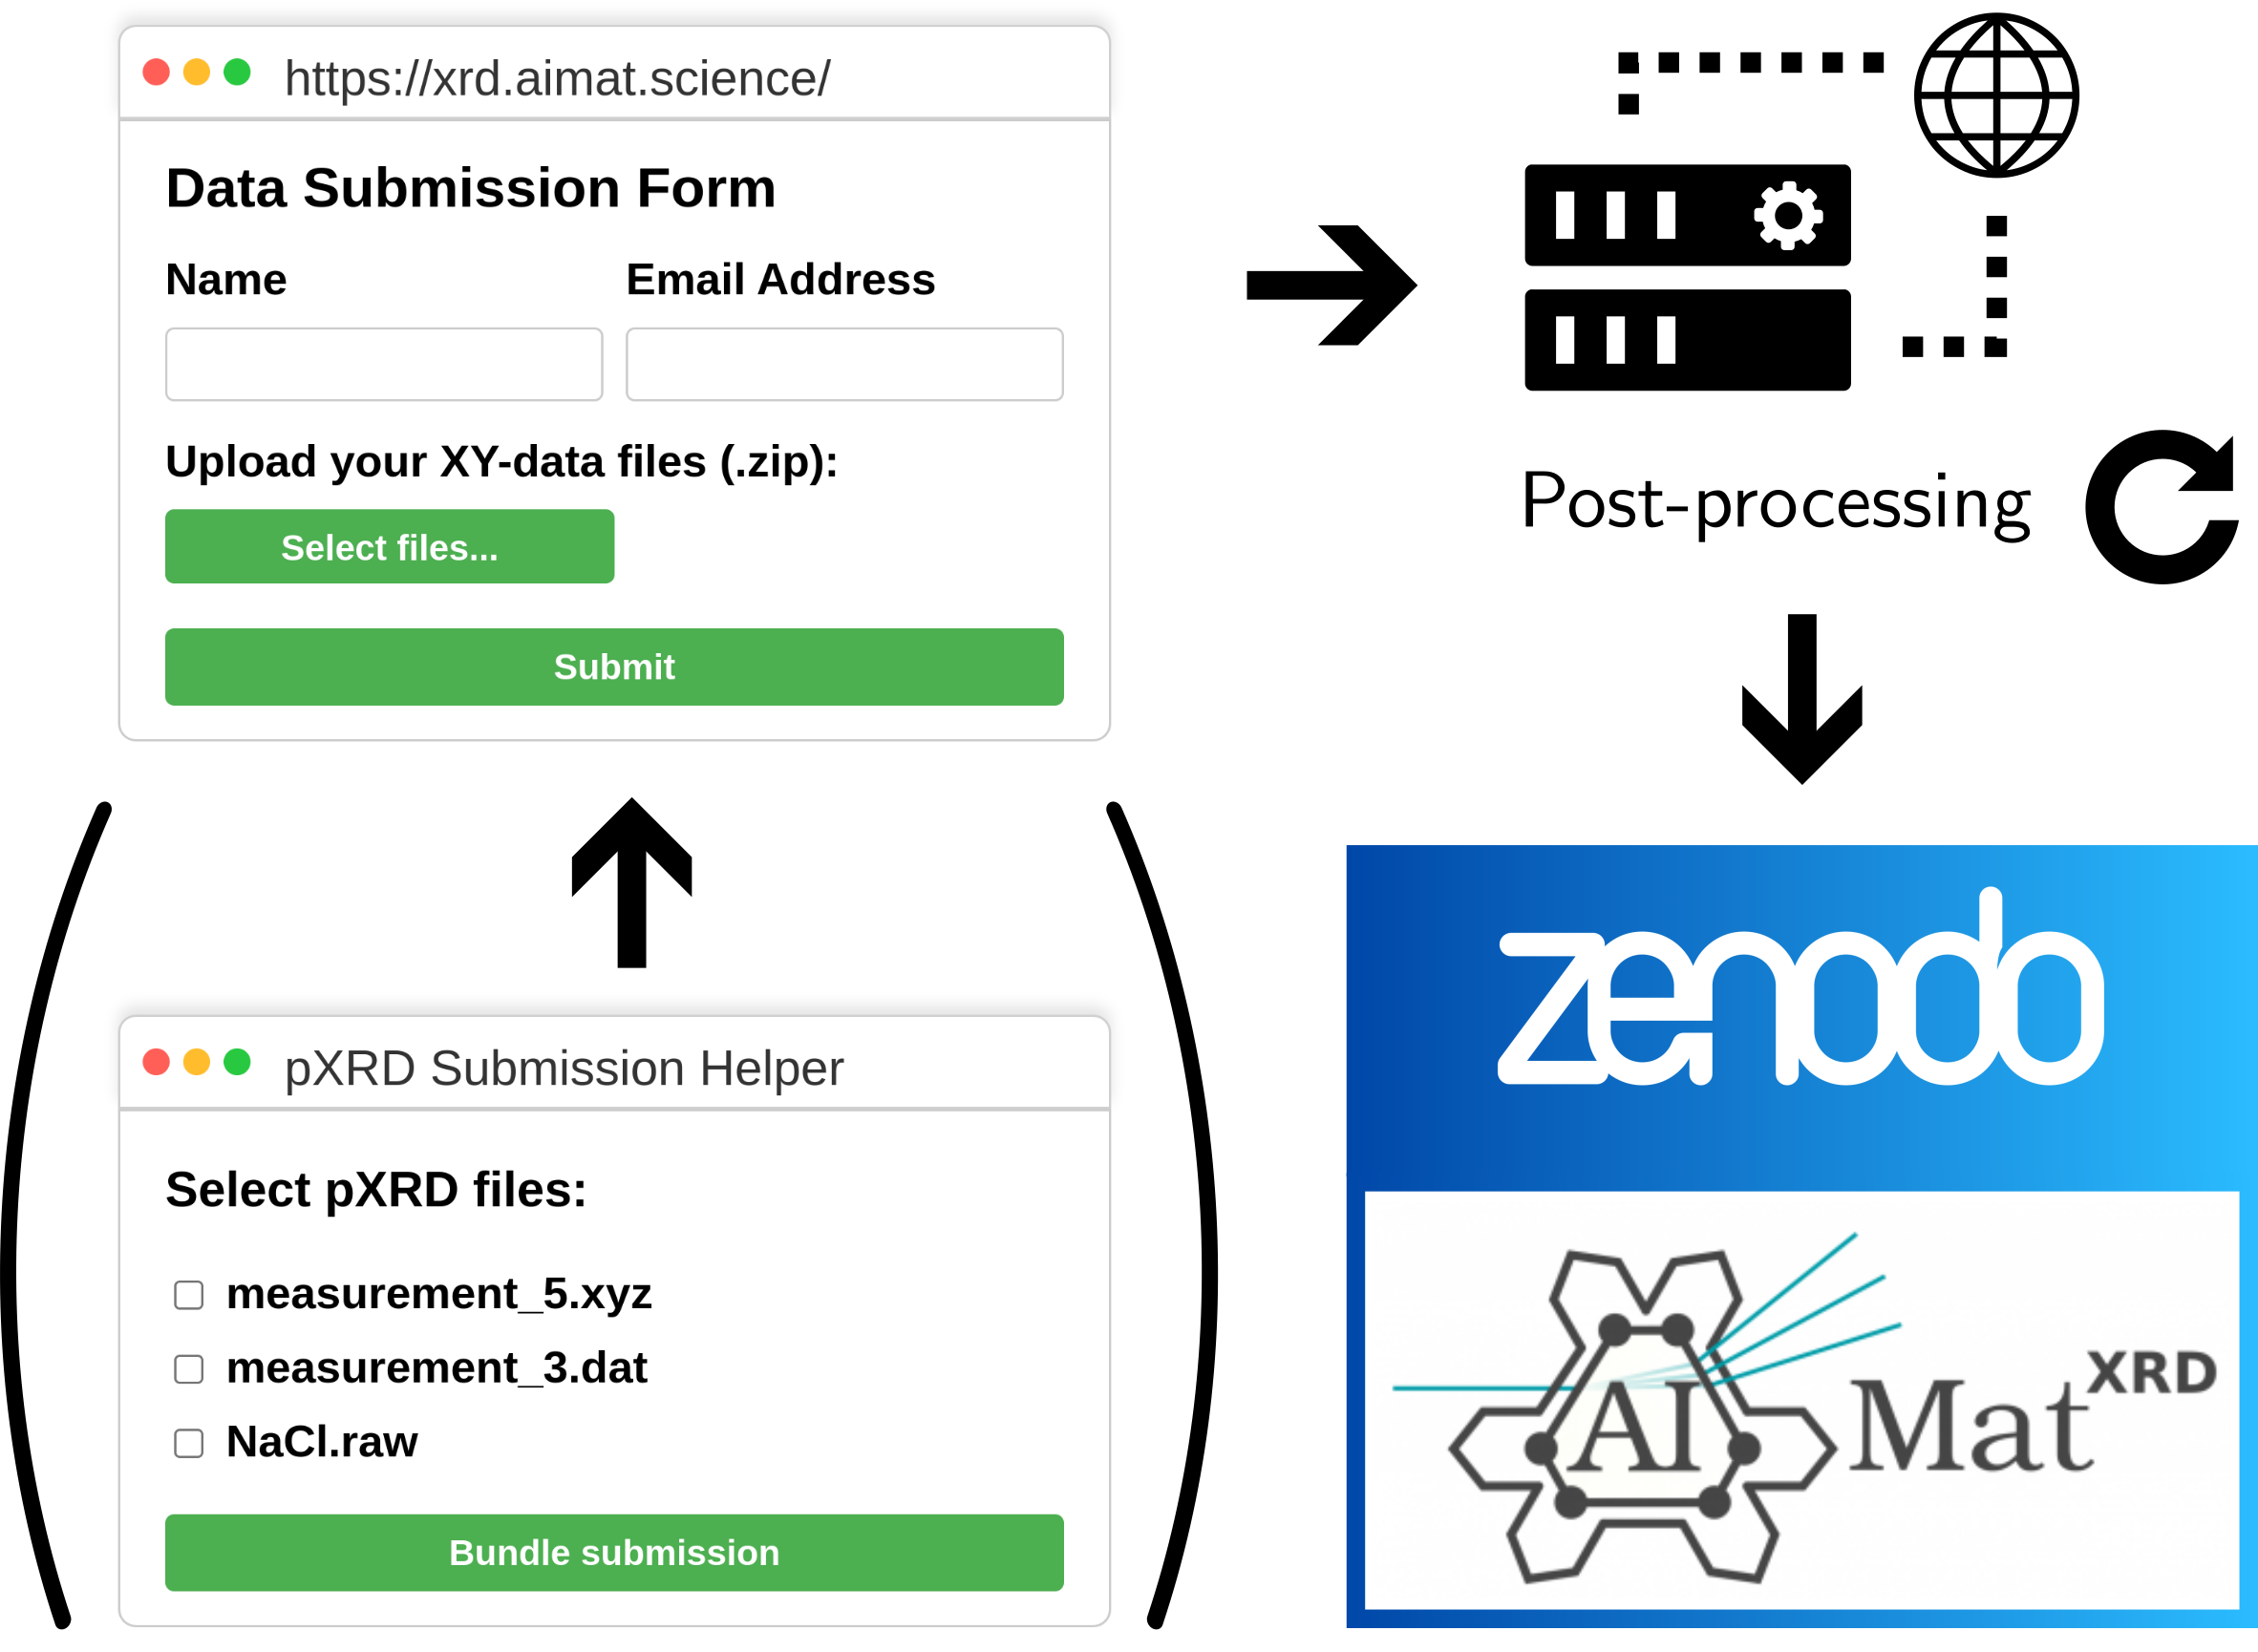
\includegraphics[width=\linewidth]{figures/overview2.png}
    \caption{Overview of the data collection pipeline. Datasets are submitted using an online submission form or our submission helper software. After post-processing and data homogenization, we create a Zenodo entry for each user submission and subsequently include the submission in the opXRD database.}
    \label{fig:overview}
\end{figure*}

% How to contribute? This aspect deserves a separate paragraph
The opXRD database is planned as a growing, community-driven initiative. The dataset we present here is the first version, but we hope to further increase the dataset size through active engagement with the pXRD community. Our primary objective is to minimize the effort and thus the barrier to contributing experimental data to the opXRD database. Thus, we developed a program that helps to find and share data from e.g. pXRD lab computers. In detail, users can select their most common pXRD file types, the program lists all files of that type, and users can select or deselect certain folders or files for sharing. Selected contributions will be uploaded to opXRD, processed to a common file format, and - if wanted - published on Zenodo on behalf of the contributors, before becoming part of the opXRD database. If labels are available, they can be shared with opXRD as well. Further details can be found on the opXRD website (Figure~\ref{fig:overview}). \\

As argued by Aranda and Kroon-Batenburg \textit{et al}.\cite{Aranda2018, Kroon-Batenburg2024}, sharing raw powder diffraction data is not only in the interest of furthering machine learning research but is also in line with open science principles. It furthers the ability of other researchers to reproduce published work and in turn, adds to the credibility of the publisher of the data. Considering our streamlined submission and post-processing framework, a publication of powder diffraction data through the opXRD database is a simple way of realizing these principles. Compared to uploading the data to Zenodo it also has the added benefit that the data is contributed towards a large, homogenous dataset with a standardized interface. This makes the data more easily accessible to other researchers and provides more value to researchers seeking great quantities of data compared to an isolated submission on Zenodo. \\


The broad range of available experimental samples contained in the opXRD v1.0 database makes it possible to apply state-of-the-art ML approaches to the domain of powder XRD analysis. We hope that this can drive ML research in this field towards more advanced automated analysis workflows that can accelerate material science research through ready application in high-throughput experimentation pipelines.

% Existing datasets (and why they dont cut it)
\section{Existing datasets}\label{sec:existing_datasets}

%% Datset listing (List written on 20.06.24)
% Lists of Crystallographic databases; Our list contains all of the databases given in the lists linked below
% - IUCR: "Crystallographic databases and related resources" (https://www.iucr.org/resources/data/databases)
% - Bruno et al. (2017): "Crystallography and Databases" (https://datascience.codata.org/articles/10.5334/dsj-2017-038)
% - University of Virginia "Crystallographic data" (https://guides.lib.virginia.edu/c.php?g=514782&p=3568808)

% [X] 1 PDF5+ (https://www.icdd.com/,https://www.icdd.com/pdf-5/) -> 19000 structures with pXRD patterns | I checked with their support
    % (1.1): ICDD Powders
    % (1.2): FIZ ICSD (https://icsd.products.fiz-karlsruhe.de/)
    % (1.3): NIST ICSD https://icsd.nist.gov/
    % (1.4): Linus Pauling File (https://paulingfile.com/index.php?p=about%20us)
    % (1.5): ICDD Single Crystal data
% [x]: 2 COD (https://www.crystallography.net/cod/) -> ~ 1000 structures with real pXRD patterns | These patterns were extracted by PSL university
% [x]: 3 RRUFF (American Mineralogist Crystal Structure Database) -> ~ 1000 structures with real pXRD patterns | We downloaded the entire dataset and discarded single crystal data
% [x]: 4 CCDC (https://www.ccdc.cam.ac.uk/) -> No exp pXRD | There is only mention of simulated powder diffraction data. Of 20 sampled cifs none contained powder diffraction data
% [x]: 5 The Material Project (https://legacy.materialsproject.org/) -> No exp pXRD | The only mention of available X-ray diffraction data is of simulated data
% [x]: 6 Crystal Lattice Structures (https://www.atomic-scale-physics.de/lattice/) -> No exp pXRD | Their entries provide no X-ray diffraction data, and also most links appear broken
% [x]: 7 Crystallographic and Crystallochemical Database for Minerals and their Structural Analogues (https://database.iem.ac.ru/mincryst/) -> No exp pXRD | The given powder diffraction data is simulated (see: Powder X-ray Diffraction Standards (CPDS) @ https://database.iem.ac.ru/mincryst/descript.htm)
% [x]: 8 Mineralogy Database (https://webmineral.com/) -> No exp pXRD | I checked with the author of the site
% [x]: 9 IUCr Raw data letters (https://iucrdata.iucr.org/) -> No exp pXRD | There are only two raw data letters, both of them single crystal data
% [x]: 10 Bilbao Crystallographic server  (https://www.cryst.ehu.eus/bincstrdb/search/) No exp pXRD | Of 20 sampled CIFs out of 256 entries none contained pXRD data
% [x]: 11 PowBase (http://www.cristal.org/powbase/index.html) -> 169 real pXRD patterns some of which have at least partial labels; The described submission process and the lack of crystal structures indicate that the patterns are not simulated
% [x]: 12 Athena (https://athena.unige.ch/athena/mineral/mineral.html) -> No exp pXRD | No mention of diffraction data anywhere
% [x]: 13 Protein database (https://www.rcsb.org/) / NAKB (https://www.nakb.org/) / BMCD ((http://bmcd.ibbr.umd.edu/)  -> Little to no exp pXRD | Of the 230k structures only 21 showed up when searching experimental method = Powder diffraction
% [x]: 14 Crystal Met (https://cds.dl.ac.uk/cds/datasets/crys/mdf/llmdf.html) -> No exp pXRD | The only mention of diffraction data is simulated data
% [x]: 15 Pearson's Crystal data (https://www.crystalimpact.com/pcd/) -> 21700 experimental powder diffraction patterns (As per https://www.crystalimpact.com/pcd/) | The Pearson's crystal data evolved from the Linus Pauling File which is a data source of the PDF, so there may be significant overlap in these patterns
% [x]: 16 Zenodo powder diffraction data (https://zenodo.org/search?q=powder%20diffraction&l=list&p=1&s=10&sort=bestmatch) -> Some pXRD data but hard to quantify, probably <= 4000 patterns most of which are unlabeled | 1600 datasets matching "powder diffraction". From probing among the first 100 matches I estimate only about 1 in 10 contain powder diffraction patterns. The probed datasets that did contain powder diffraction data only contained <= 30 patterns and only one of them came with corresponding crystal structures

%TODO: Summarize the existing datasets shortly, including number of entries, etc.

\pagebreak

\subsubsection*{Existing experimental powder diffraction datasets}
To contextualize opXRD within the current environment of experimental powder diffraction data, the following list provides an overview of the largest crystal structure databases that include powder diffraction data.  \\

\textbf{Powder Diffraction File:}\footnote{More information on the Powder Diffraction File can be found under \url{https://www.icdd.com/pdf-5/}.} The Powder Diffraction File (PDF), published and maintained by the International Center for Diffraction Data (ICDD), is a large collection of materials with accompanying powder diffraction data. Its latest release as of November 2024, the PDF5+, contains over a million materials with accompanying powder diffraction data. However, most of these powder diffraction patterns are simulated. After inquiring with the ICDD in April 2024 we were told that only 19000 of the powder diffraction patterns in the PDF5+ stemmed from experiments. \footnote{We reached out to the contact address given on their website, info@icdd.com.} Still, this makes the PDF5+, to the best of our knowledge, the largest collection of experimental powder diffraction data available to researchers. As of November 2024, the PDF5+ is available to researchers through a purchase starting at a price point of \$6,265.00.\\

\textbf{Crystallography Open Database:}\footnote{More information on the crystallography open database can be found under \url{https://www.crystallography.net/cod/}.} The Crystallography Open Database (COD)\cite{Graulis2009cod} is an open-access collection of crystal structures. It provides over 500.000 crystal structures in the form of .cif files. Of these files, 1063 contained the experimental powder diffraction data that was used to determine the underlying crystal structures of the investigated samples. \\

\textbf{RRUFF}: The RRUFF Mineral Database \cite{Armbruster2015} provides detailed information on minerals, including their chemical compositions, crystallography, and spectroscopic data. Managed by the University of Arizona, it was created to serve as a public repository for mineral identification and research. It contains \num{908} distinct structures with experimental x-ray diffraction patterns. \\

\textbf{PowBase}: 

\textbf{Pearson's Crystal data}:

Some major crystal structure databases, such as the ICSD, do not appear in the above list, as they do not include powder diffraction data. This is because most structure solutions are achieved through single-crystal diffraction rather than powder diffraction.
 

% Our dataset (and why its better)
\section{Our dataset}\label{sec:our_dataset}
%% Notes:
% The subsections of this section should be the 
% individual contributions that we get from labs

% Sharing raw powder x-ray diffraction data: Challenges and benefits https://www.researchgate.net/publication/329256004_Sharing_powder_diffraction_raw_data_Challenges_and_benefits

In collaboration with several other institutions we have collected a dataset of diffractograms stemming from experiment, some of them labeled with corresponding structural information. \\
Currently, institutions that contributed towards our dataset include:
\item Institute of Nanotechnology at Karlsruhe institute of technology
\item University of Southern California
\item Lawrence Berkeley National Laboratory

We are still in the process of growing the dataset and additional contributions are still very welcome. 
To find out more about how to contribute to this dataset, visit our website specially designed for the purpose of collecting this dataset, https://xrd.aimat.science \\

A major advantage of this dataset over other comparable datasets is that is is very easy to handle in python and in PyTorch. \\
Our accompanying python library xrdpattern (https://github.com/aimat-lab/xrdpattern) provides a means to read in as much of the dataset as fits in memory simply by using PatternDB.load(data_dirpath). The patterns attribute of this class is a list of the indivdual pattern diffractograms, each of which supports a standardize, plot and to tensor method. \\
The standardize method returns a "standardized" version of the pattern with a fixed angle range, a fixed number of entries and intensities normalized to the $[0,1]$ interval.




\printnomenclature

\clearpage

%\listofchanges
%\clearpage

%\nocite{*}
%\TheBibliography
%\printbibliography[heading=bibintoc]

\bibliography{bib}
\bibliographystyle{rsc} %the RSC's .bst file

\end{document}